\documentclass[12pt,a4paper]{article}

\usepackage{times}
\usepackage{lipsum} %para gerar alguns textos como exemplo

%\usepackage[brazil]{babel} %para portugues brasil
\usepackage[brazil,brazilian]{babel}
\usepackage[T1]{fontenc} 
\usepackage[utf8]{inputenc}

\usepackage{color,graphicx} %permite a inserção de figuras
\usepackage{lineno} %usamos este pacote para retirar o espaço em branco ao redor das figuras

\usepackage{setspace} %espaçamento entre linhas (doublespacing, singlespacing)
\usepackage[top=3cm,left=3cm,right=2cm,bottom=2cm]{geometry} %definir margens
%\setlength{\columnsep}{1cm}

%%O pacote abaixo serve para inserir códigos
\usepackage{listings}% http://ctan.org/pkg/listings
\lstset{
  basicstyle=\ttfamily,
  mathescape
}
%%%%%%%%%%%%%%%%%%%%%%%%%%%%%%%%%%%%%%%%%%%%%%%%%%%%
% Renomeando as palavras do pacote BABEL - BRAZILIAN
%%%%%%%%%%%%%%%%%%%%%%%%%%%%%%%%%%%%%%%%%%%%%%%%%%%%
\addto\captionsbrazilian{%
  \renewcommand{\contentsname}%
    {\centering SUMÁRIO} % Sumário para SUMÁRIO
  \renewcommand{\figurename}%
    {FIGURA} % Figura para FIGURA
  \renewcommand{\tablename}%
    {TABELA} % Tabela para TABELA
  \renewcommand{\listfigurename} %
    {\centering LISTA DE FIGURAS} %Lista de Figuras para LISTA DE FIGURAS
  \renewcommand{\listtablename} %
    {\centering LISTA DE TABELAS} %Lista de Tabelas para LISTA DE TABELAS
}

%% FORMATAÇÃO DO INDICE
%%
\usepackage{etoolbox}
\makeatletter
\patchcmd{\l@section}
  {\hfil}
  {\leaders\hbox{\normalfont$\m@th\mkern \@dotsep mu\hbox{.}\mkern \@dotsep mu$}\hfill}
  {}{}
\makeatother
%% FIM FORMATAÇÃO DO INDICE
\begin{document}
%%
%% ********** CAPA
%%

%% não numerar a página
\thispagestyle{empty}
%\hyphenation{Graduação título Lavras concentração obtenção exigências Sistemas}

\begin{center}


\includegraphics[scale=0.5]{figuras/logo_cefet.png}

\vspace{0.5in}

CENTRO FEDERAL DE EDUCAÇÃO TECNOLÓGICA DE MINAS GERAIS

\vspace{0.5in}

GRADUAÇÃO EM ENGENHARIA ELÉTRICA

\vspace{1.0in}

{\Large \textbf{CÁLCULO DO PERFIL TRANSVERSAL DO CAMPO MAGNÉTICO DE LINHAS DE TRANSMISSÃO DE ALTA TENSÃO}}

\end{center}

\vspace{1.8in}

\begin{flushleft}
\textbf{ALUNOS:} \\
FULANO\\
CICLANO\\
BELTRANO

\textbf{PROFESSOR:} FULANO DE TAL

\textbf{DISCIPLINA: } LABORATÓRIO DE ELETROMAGNETISMO
\end{flushleft}

\vspace{0.8in}

\begin{center}
\textbf{NEPOMUCENO}\\
\textbf{OUTUBRO/2015} %\\ \vspace{2ex}

\end{center}


%%%%%%%%%%%%%%% FIM DA CAPA %%%

%%
%% ********** SUMARIO
%%

\newpage
\thispagestyle{empty}
\tableofcontents


%%
%% ********** CORPO DO DOCUMENTO
%%

\newpage

%\pagestyle{myheadings}
\setcounter{page}{1}
\section{Introdução}
\lipsum[1-2]

\begin{figure}[h!]
\centering 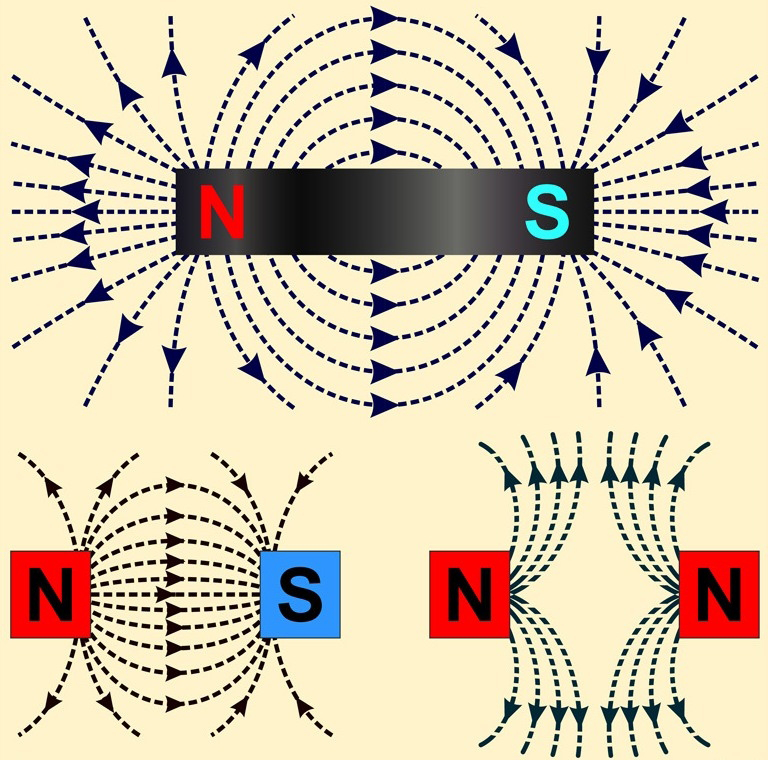
\includegraphics[scale=0.3]{figuras/figura1.png}
\caption{Blá blá blá} \label{fig:fig1}
\end{figure}
\lipsum[1-1]

Assim podemos observar que o sentido adotado para o campo magnético é sempre do pólo
norte do imã para o pólo sul.

A intensidade do campo magnético $(\vec{H})$ em um ponto $P (Xp,Yp,Zp)$ devido a uma corrente que
percorre um condutor filamentar retilíneo de comprimento infinito é determinada pela equação :

\begin{equation}
\vec{H} = \frac{I}{2\pi \rho }\hat{a}_{\phi} 
\label{eq:eq1}
\end{equation}

Observe que H está sempre ao longo do vetor unitário $\hat{a}_{\phi}$, isto é, em trajetórias circulares
e concêntricas.

Encontrar o vetor unitário $\hat{a}_\phi$ na Equação \ref{eq:eq1} nem sempre é fácil. Uma abordagem simples
é determinar $\hat{a}_{\phi}$ de $a_{\phi} = a_1 \chi a_{\rho}$ onde $a_l$ é o vetor unitário ao longo da corrente em uma linha e $a_\rho$ é o vetor unitário ao longo da linha perpendicular traçada a partir da corrente até o ponto onde se quer calcular o campo .

\newpage
\section{Metodologia}

\lipsum[1-3]

\begin{equation}
I = \frac{S}{\sqrt{3} \ast V_1}
\label{eq:eq2}
\end{equation}

\lipsum[1-1]

\begin{figure}[!h]
\centering 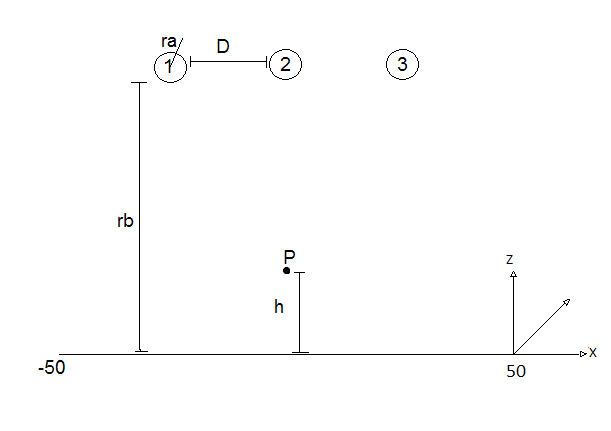
\includegraphics[scale=0.5]{figuras/figura2.png}
\caption{Outro blá} \label{fig:fig2}
\end{figure}

\lipsum[1-1]


\subsection{Algoritmo comentado}

\begin{lstlisting}
clc;
clear all;
S = input('Potencia: '); //Leitura da potencia
V=input('Tensao entre fases: '); //Leitura da tensao.
//Leitura da altura das fases ao solo.
h=input('Altura da fase ao solo: '); 
//Leitura da altura do ponto ao solo.
hzin=input('Altura do ponto: ');
//Separacao entre as fases.
separacao=input('Distancia entre fases: '); 
I=S/(sqrt(3)*V); //Calculo da corrente.
I1=I;
c=(-0.5+i*0.866); //Parte complexa da corrente B.
d=(-0.5-i*0.866); //Parte complexa da corrente C.
I2=I*c;
I3=I*d;
perfil=[-50:50]; // Variacao no eixo x.
for i=1:101

//Calculo do campo para todas as fases no eixo Z.
Hz(i)=(I1*(-(perfil(i)+separacao)))/
(2*3.1415*(((perfil(i)+separacao)^2)+
((hzin-h)^2)))+(I2*-(perfil(i)))/
(2*3.1415*(((perfil(i))^2)+((hzin-h)^2)))+
(I3*(-(perfil(i)-separacao)))/
(2*3.1415*(((perfil(i)-separacao)^2)+
((hzin-h)^2))); 

//Calculo do campo para todas as fases no eixo x.
Hx(i)=(I1*(hzin-h))/
(2*3.1415*(((perfil(i)+separacao)^2)+
((hzin-h)^2)))+(I2*(hzin-h))/
(2*3.1415*(((perfil(i))^2)+((hzin-h)^2)))+
(I3*(hzin-h))/(2*3.1415*
(((perfil(i)-separacao)^2)+
((hzin-h)^2))); 

//Modulo do campo no eixo z.
Hz(i)=sqrt(((real(Hz(i)))^2)+((imag((Hz(i)))))^2); 
//Modulo do campo no eixo x.
Hx(i)=sqrt(((real(Hx(i)))^2)+((imag((Hx(i)))))^2); 
// Calculo do campo resultante.
Hw(i)=sqrt(((Hx(i))^2)+((Hz(i)))^2); 
end
plot(perfil,Hw); //Geracao do grafico 2D.
\end{lstlisting}

\newpage
\section{Resultados e conclusão}
\lipsum[1-1]
Na Figura \ref{fig:fig3}, temos:

\begin{figure}[!ht]
\centering 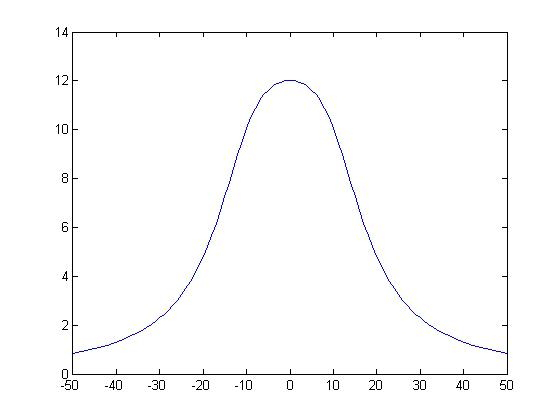
\includegraphics[scale=0.5]{figuras/figura3.png}
\caption{Conclusão} \label{fig:fig3}
\end{figure}

\lipsum[1-1]

\newpage
%\addcontentsline{toc}{section}{\hspace{1.5 em}Referências}
\section{Referências}

\singlespacing COSTA, Eduard Montgomery Meira; DARCEY, Lauren. C Aplicado ao Aprendizado de
Eletromagnetismo. Rio de Janeiro: Ciencia Moderna, 2012.

\doublespacing 

\singlespacing \noindent SADIKU, Matthew N. O. Elementos de Eletromagnetismo. 5ª ed. Bookman, 2012.
\end{document}